\subsubsection{Extension 5}
\begin{namedframe}{Angles subtended by the same arc}
	\begin{example}
		Show that if $C_1$ and $C_2$ are two different choices for the position of the point $C$ along the same arc $AB$ then $\angle AC_1B = \angle AC_2B$.
		\vertspace
		This is equivalent to saying that angles subtended by the same arc are equal.
	\end{example}
	\pause
	\centering
	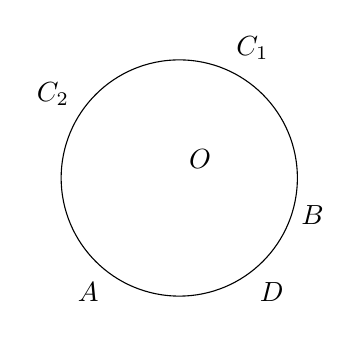
\begin{tikzpicture}[scale=0.3]
		\coordinate [label=above right:$O$](O) at (0,0);
		\coordinate [label=below left:$A$](A) at (-3,-4);
		\coordinate [label=right:$B$](B) at (4.75,-1.5612494996);
		\coordinate [label=above right:$C_1$](C1) at (2,4.58257569496);
		\coordinate [label=above left:$C_2$](C2) at (-4.25,2.63391343821);
		\coordinate [label=below right:$D$](D) at (3,-4);

		\draw (O) circle (5);
	\end{tikzpicture}
	\pause
	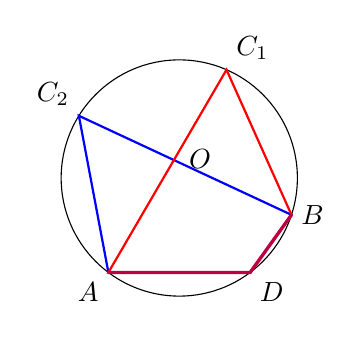
\begin{tikzpicture}[scale=0.3]
		\coordinate [label=above right:$O$](O) at (0,0);
		\coordinate [label=below left:$A$](A) at (-3,-4);
		\coordinate [label=right:$B$](B) at (4.75,-1.5612494996);
		\coordinate [label=above right:$C_1$](C1) at (2,4.58257569496);
		\coordinate [label=above left:$C_2$](C2) at (-4.25,2.63391343821);
		\coordinate [label=below right:$D$](D) at (3,-4);

		\draw (O) circle (5);
		\draw [blue,thick] (A) -- (C2) -- (B) -- (D) -- cycle;
		\draw [red,thick] (A) -- (C1) -- (B) -- (D) -- cycle;
		\draw [purple,very thick] (A) -- (D) -- (B);
	\end{tikzpicture}
\end{namedframe}
\begin{namedframe}{Extension 5 proof}
	\begin{proof}[Proof that $\angle AC_1B = \angle AC_2B$.]
		\begin{wrapfigure}{l}{0pt}
			\scriptsize
			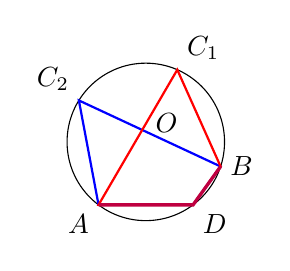
\begin{tikzpicture}[scale=0.2]
				\coordinate [label=above right:$O$](O) at (0,0);
				\coordinate [label=below left:$A$](A) at (-3,-4);
				\coordinate [label=right:$B$](B) at (4.75,-1.5612494996);
				\coordinate [label=above right:$C_1$](C1) at (2,4.58257569496);
				\coordinate [label=above left:$C_2$](C2) at (-4.25,2.63391343821);
				\coordinate [label=below right:$D$](D) at (3,-4);

				\draw (O) circle (5);
				\draw [blue,thick] (A) -- (C2) -- (B) -- (D) -- cycle;
				\draw [red,thick] (A) -- (C1) -- (B) -- (D) -- cycle;
				\draw [purple,very thick] (A) -- (D) -- (B);
			\end{tikzpicture}
		\end{wrapfigure}
		Using extension 4, we know that:
		\pause
		\[\angle AC_1B + \angle ADB = \SI{180}{\degree}\]
		\pause
		\[\angle AC_2B + \angle ADB = \SI{180}{\degree}\]
		\sep[5ex]
		So:
		\pause
		\begin{align*}
			\angle AC_1B + \angle ADB &= \angle AC_2B + \angle ADB\\
			\angle AC_1B &= \angle AC_2B \qedhere
		\end{align*}
	\end{proof}
\end{namedframe}
